\chapter{Применение описанных подходов на практике}

В настоящей главе описывается эксперимент, в котором применялся
подход, описанный в главе~\ref{ch:problem_solving}, на
конкретной задаче определения демографических характеристик
пользователей с использованием конкретного набора данных.

В разделе~\ref{sec:dataset} произведён обзор набора данных,
который использовался в эксперименте, а также описана
конкретная задача, которая решалась.

В разделе~\ref{sec:algorithms_config} описаны применяемые
алгоритмы, а также их конфигурация.

В разделе~\ref{sec:result_quality} описан способ измерения
качества результата.

Наконец, в разделе~\ref{sec:results} приведены результаты,
полученные в проведённом эксперименте.

\section{Описание набора данных}
\label{sec:dataset}

Для подтверждения состоятельности описанного подхода к решению задачи
профилирования пользователей на основе анализа их музыкальных
интересов был проведён эксперимент. Решалась задача определения
демографических характеристик (пола и возраста) пользователей сайта 
Last.fm с использованием набора данных, который использовался в
работе~\cite{wu2014gender}.

Авторы упомянутой работы загружали данные с сайта Last.fm. Всего набор
данных содержит 96807 пользователь. Для каждого пользователя была
получена информация о его музыкальных интересах при помощи метода
публичного API сайта \textit{User.getTopTracks}, который возвращает
50 наиболее прослушиваемых музыкальных композиций заданным пользователем. 
Музыкальные композиции отсортированы в порядке убывания числа прослушиваний.
При этом данные содержат только имена исполнителей, извлечённые из этого списка.
То есть данные имеют такой вид, который был описан в 
разделе~\ref{sec:problem_formulation}. 

Кроме того, при помощи метода API сайта \textit{User.getInfo}
была получена информация о поле и возрасте для каждого пользователя.

Каждый пользователь в наборе описан по меньшей мере 40
музыкальными композициями. У каждого пользователя указан пол и возраст.
Набор данных содержит 133938 уникальных музыкальных исполнителей.

Стоит также отметить некоторые особенности выборки пользователей.
Во-первых, мужчин в ней содержится больше, чем женщин. Распределение
пола в выборке проиллюстрировано на рисунке~\ref{fig:gender_pie}.
Во-вторых, распределение возраста в выборке не является равномерным,
и оно смещено в сторону молодого поколения. Медиана распределения
возраста в выборке равна 31, а средний возраст равен 29,05.
Распределение возраста в выборке пользователей изображено на
рисунке~\ref{fig:age_histogram}.

Используя данные о музыкальных исполнителях пользователей,
решалось две задачи~--- задача определения пола и задача
определения возраста. Первая задача решалась как задача
бинарной классификации, а вторая~--- как задача восстановления
регрессии.

\begin{figure}[!h]
\caption{Распределение пола в выборке пользователей}
\label{fig:gender_pie}
\centering
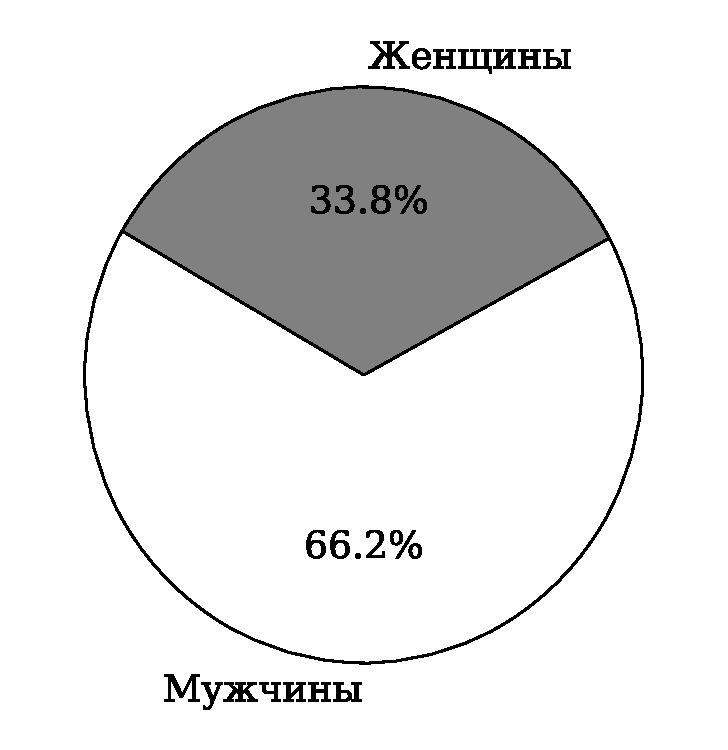
\includegraphics[scale=0.65]{figs/gender-pie.pdf}
\end{figure}

\begin{figure}[!h]
\caption{Распределение возраста в выборке пользователей}
\label{fig:age_histogram}
\centering
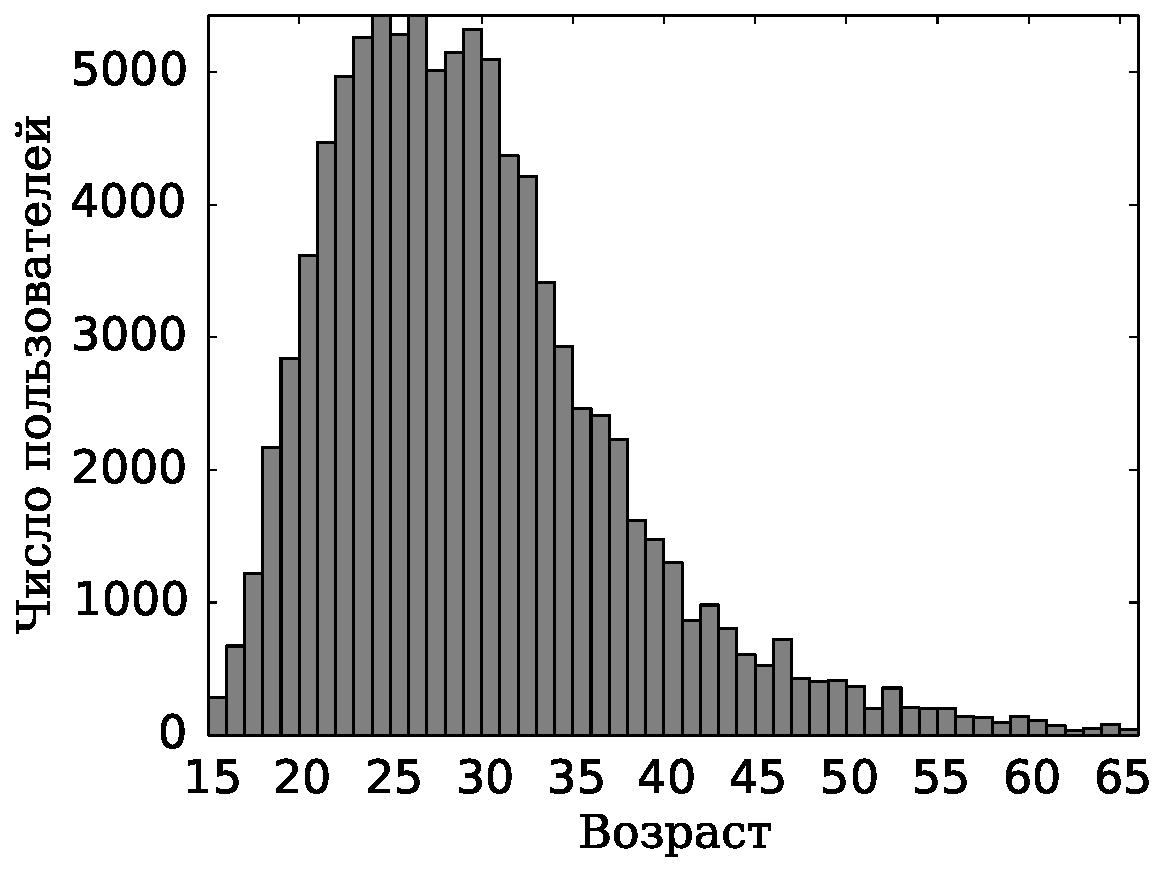
\includegraphics[scale=0.60]{figs/age-histogram.pdf}
\end{figure}

\section{Используемые алгоритмы и их конфигурация}
\label{sec:algorithms_config}

В данном разделе описаны используемые алгоритмы латентного
семантического анализа, техники word embedding, а также методов
классификации и восстановления регрессии. Кроме всего, приведены
конфигурации алгоритмов.

\subsection{Алгоритмы латентного семантического анализа}

В качестве алгоритмов латентного семантического анализа
в эксперименте использовались алгоритмы PLSA (реализация из библиотеки
\textit{BigARTM}~\cite{bigartm}), LDA (реализация из библиотеки
\textit{gensim}~\cite{gensim}) и LSI (реализация из библиотеки
\textit{gensim}).

Стоит отметить, что при использовании алгоритмов
\textit{PLSA} и \textit{LDA} результаты получались похожими 
на случайные, поэтому детальные эксперименты с их 
использованием не проводились. 

Возможно, такое поведение объясняется тем фактом, 
что их использование основано на гипотезе о существовании 
латентных жанров исполнителей, но часто не существует единогласного 
мнения о жанрах, которые исполняет тот или иной музыкальный исполнитель.
Поэтому можно считать, что данная гипотеза не выполняется.

Также имеет место предположение о том, что в большинстве случаев
люди предпочитают слушать музыку различных жанров, поэтому жанры
являются неинформативными признаками.

Напротив, использование алгоритма \textit{LSI} позволяет получить хорошие
результаты. Именно он и использовался в детальных экспериментах, результаты
которых будут приведены в разделе~\ref{sec:results}.

Для параметра алгоритма \textit{LSI}, характеризующего число тематик,
использовалось два значения~--- 20 тематик и 200 тематик. 
Для остальных параметров алгоритма использовались значения по умолчанию.

\subsection{Алгоритмы векторного представления слов}

В качестве алгоритма, реализующего модель векторного представления
слов, использовался алгоритм Word2Vec, а именно его реализация из
библиотеки \textit{gensim}.  

В качестве размерности векторов использовалось два значения~--- 200
и 20 (параметр \textit{size}).

Шириной контекста было выбрано значение 50 (параметр \textit{window}),
что означает использование в качестве контекста всех исполнителей для
любого из пользователей.

Для остальных параметров алгоритма Word2Vec использовались значения
по умолчанию.

\subsection{Алгоритмы классификации и восстановления регрессии}

В качестве алгоритма классификации или восстановления регрессии
использовался \textit{метод опорных векторов (Support Vector Machine,
SVM)}~\cite{cortes1995support} с ядром 
\textit{radial basis function (RBF)}. Использовалась реализация
метода опорных векторов из программной библиотеки 
\textit{scikit-learn}~\cite{sklearn}, а именно алгоритмы
\textit{SVC} и \textit{SVR} для задач классификации и регрессии
соответственно. Данные алгоритмы основаны на реализации
из программной библиотеки \textit{LibSVM}~\cite{libsvm}.

Параметры метода опорных векторов \textit{C} и \textit{gamma},
выбор которых во многих задачах сильно влияет на результат,
настраивались на обучающей выборке (подробнее о разбиении
на обучающую и контрольную выборку см.
раздел~\ref{sec:result_quality}) методом \textit{GridSearchCV},
который реализован в библиотеке \textit{scikit-learn}. Множества
параметров \textit{C} и \textit{gamma} были выбраны следующие:
\[
    C \in \{0; 1; 0{,}5; 1; 3\},\quad
    \mathrm{gamma} \in \{0{,}001; 0{,}01; 0{,}1; 1; 8; 16; 32; 64\}.
\]

Метод \textit{GridSearchCV} использует \textit{кросс-валидацию}
с разбиением на $k$ частей (\textit{k-fold cross validation}).
Было выбрано число разбиений равное трём.

Для задачи определения пола параметры подбирались таким
образом, чтобы максимизировать точность классификации (подробнее
см. раздел~\ref{sec:result_quality}).

Для задачи определения возраста параметры подбирались так, чтобы
минимизировать среднюю абсолютную ошибку (подробнее см.
раздел~\ref{sec:result_quality}).

Перед использованием алгоритма классификации или регрессии
вектора пользователей были нормализованы по $L_2$ норме
(при использовании латентного семантического анализа) или
стандартизованы (при использовании подхода на основе
векторного представления слов).

\section{Способ измерения качества результата}
\label{sec:result_quality}

Разбиение выборки пользователь на обучающую и контрольную
было произведено случайным образом, но так, чтобы распределение
пола в каждой из выборок было одинаковым.

Обучающая выборка содержит 48404 пользователей, а контрольная~---
48403 пользователей.

Стоит отдельно отметить, что разбиение выборки пользователей на
обучающую и контрольную было произведено \textit{в точности таким
же образом}, как это было сделано в работе~\cite{wu2014gender}.

Обучение происходило на обучающей выборке, а качество классификации
или восстановления регрессии измерялось на контрольной выборке
с использованием метрик. Опишем этим метрики. 

Пусть имеется матрица <<пользователь-признак>>
$X \in \mathbb{R}^{n \times m}$. Будем обозначать вектор,
описывающий пользователя $i$ как $\bm{x}_i$ (строка матрицы $X$).
Множество этих векторов будем обозначать как $\mathcal{X}$.
Также пусть для каждого пользователя с номером $i$ имеется метка,
обозначающая пол пользователя $g_i \in G$ и метка, обозначающая
возраст~--- $a_i \in A$. Тогда метрика для определения качества
классификации (называемая \textit{точностью}) будет иметь следующий вид:
\[
    \mathrm{ACC} = 
    100\% \cdot \frac{1}{n} \cdot 
    \sum_{i=1}^{n}[g_i = \mathcal{C}(\bm{x}_i)],
    \quad \mathcal{C} \colon \mathcal{X} \mapsto G,
\]
где $\mathcal{C}$~--- алгоритм классификации. А метрика для оценки
качества восстановления регрессии (называемая \textit{средней
абсолютной ошибкой}) вычисляется по формуле:
\[
    \mathrm{MAE} =
    \frac{1}{n} \cdot \sum_{i=1}^{n} 
    \left|a_i - \mathcal{R}(\bm{x}_i)\right|,
    \quad \mathcal{R} \colon \mathcal{X} \mapsto A,
\]
где $\mathcal{R}$~--- алгоритм восстановления регрессии.

Большое значение точности характеризует высокое качество классификации.
Малое значение средней абсолютной ошибки характеризует высокое качество
восстановления регрессионной зависимости.

Ввиду того, что распределение пола в выборке пользователей
является неравномерным, в результатах также будут приведены
\textit{матрицы ошибок (error matrix, confusion matrix)
}~\cite{stehman1997selecting} для задач классификации.
Данные матрицы показывают число верно и неверно классифицированных
объектов для каждого из классов.

\section{Результаты}
\label{sec:results}

В данном разделе приведены результаты, полученные в 
эксперименте, в котором применялся подход, описанный в 
главе~\ref{ch:problem_solving}.

В таблице~\ref{tab:bow_lsa}
приведены результаты с использованием подхода <<bag of words>>
для вычисления матрицы <<исполнитель-пользователь>> и латентного
семантического анализа для построения матрицы <<пользователь-признак>>.
Для вычисления элементов матрицы <<исполнитель-пользователь>> использовалась
обобщённая формула TF-IDF (см. формулу~\ref{eq:general_tfidf}) с
использованием различных функций $l$ и $g$, а также формула
log-entropy (см. формулу~\ref{eq:log_entropy}). Как видно,
добиться наилучших результатов позволяет простейший подход,
при котором элемент $d_{ij}$ матрицы <<исполнитель-пользователь>>
равен единице, если исполнитель $i$ встречается у пользователя $j$,
и нулю~--- иначе. Для модели, позволяющей достигнуть лучших
результатов в задаче определения пола,
на рисунке~\ref{fig:bow_lsa_conf} приведены матрицы ошибок.

\begin{table}[!h]
    \caption{Результаты эксперимента с применением подходов
            <<bag of words>> и латентного семантического анализа}
    \label{tab:bow_lsa}
\centering
\begin{tabular}{|c|c|c|c|c|}\hline
    \textbf{Формула} & \boldmath$l(x)$ & \boldmath$g(x)$ & \textbf{Определение пола} & \textbf{Определение возраста} \\\hline
    \multicolumn{5}{|c|}{\textbf{20 признаков}} \\\hline
    TF-IDF & $1$ & $1$ & \textbf{73,33\%} & \textbf{4,72} \\\hline
    TF-IDF & $\log{x}$ & $1$ & 72,83\% & 4,80 \\\hline
    TF-IDF & $\log{x}$ & $\log{x}$ & 70,56\% & 4,91 \\\hline
    TF-IDF & $\log{x}$ & $\sqrt{x}$ & 67,08\% & 5,49 \\\hline
    TF-IDF & $\sqrt{x}$ & $1$ & 72,80\% & 4,79 \\\hline
    TF-IDF & $\sqrt{x}$ & $\log{x}$ & 70,61\% & 4,91 \\\hline
    TF-IDF & $\sqrt{x}$ & $\sqrt{x}$ & 67,07\% & 5,48 \\\hline
    TF-IDF & $x$ & $1$ & 70,74\% & 5,02 \\\hline
    TF-IDF & $x$ & $\log{x}$ & 69,38\% & 5,12 \\\hline
    TF-IDF & $x$ & $\sqrt{x}$ & 67,44\% & 5,45 \\\hline
    log-entropy & --- & --- & 71,15\% & 4,90 \\\hline
    \multicolumn{5}{|c|}{\textbf{200 признаков}} \\\hline
    TF-IDF & $1$ & $1$ & \textbf{82,46\%} & \textbf{3,54} \\\hline
    TF-IDF & $\log{x}$ & $1$ & 81,59\% & 3,64 \\\hline
    TF-IDF & $\log{x}$ & $\log{x}$ & 81,67\% & 3,58 \\\hline
    TF-IDF & $\log{x}$ & $\sqrt{x}$ & 80,08\% & 5,49 \\\hline
    TF-IDF & $\sqrt{x}$ & $1$ & 72,80\% & 4,79 \\\hline
    TF-IDF & $\sqrt{x}$ & $\log{x}$ & 70,61\% & 4,91 \\\hline
    TF-IDF & $\sqrt{x}$ & $\sqrt{x}$ & 67,07\% & 5,48 \\\hline
    TF-IDF & $x$ & $1$ & 70,74\% & 5,02 \\\hline
    TF-IDF & $x$ & $\log{x}$ & 69,38\% & 5,12 \\\hline
    TF-IDF & $x$ & $\sqrt{x}$ & 67,44\% & 5,45 \\\hline
    log-entropy & --- & --- & 81,46\% & 3,59 \\\hline
\end{tabular}
\end{table}

\begin{figure}[!h]
\caption{Матрицы ошибок для задачи определения пола с
         применением подходов <<bag of words>> и
         латентного семантического анализа}
\label{fig:bow_lsa_conf}
\centering
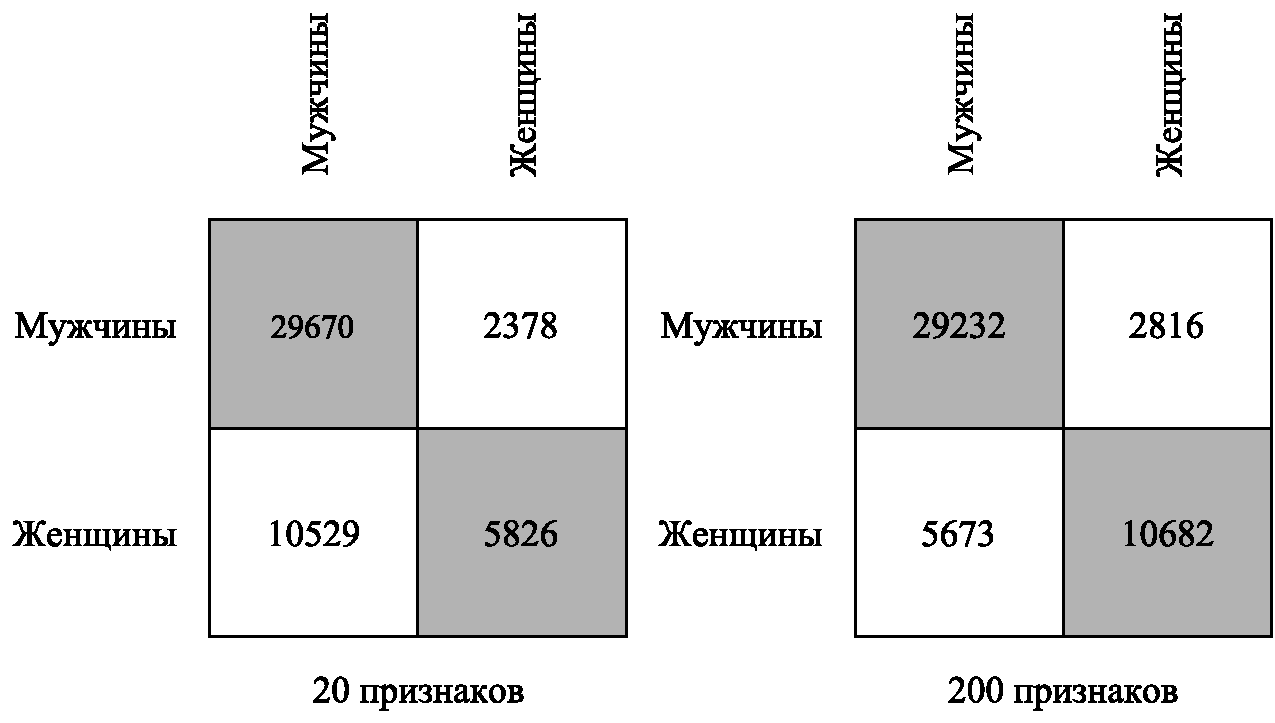
\includegraphics[scale=0.75]{figs/bow-lsa-confusion.pdf}
\end{figure}

В таблице~\ref{tab:order_lsa} приведены результаты эксперимента
с применением подхода вычисления матрицы <<исполнитель-пользователь>>
на основе порядка следования исполнителей (см. формулу~\ref{eq:order_dij})
при выборе различных функций $f$ и латентного семантического анализа.
Как видно, учёт порядка следования исполнителей только ухудшает результат.
На рисунке~\ref{fig:order_lsa_conf} приведены матрицы ошибок для 
модели, позволяющей достигнуть лучших результатов в задаче определения
пола.

\begin{table}[!h]
    \caption{Результаты эксперимента с применением подходов
             вычисления матрицы <<исполнитель-пользователь>>
             на основе порядка следования исполнителей 
             и латентного семантического анализа}
    \label{tab:order_lsa}
\centering
\begin{tabular}{|c|c|c|}\hline
    \boldmath$f(a)$ & \textbf{Определение пола} & \textbf{Определение возраста} \\\hline
    \multicolumn{3}{|c|}{\textbf{20 признаков}} \\\hline
    $\frac{1}{\log(a + 1)}$ & \textbf{71,68\%} & \textbf{4,83} \\\hline
    $\frac{1}{\sqrt{a}}$ & 71,56\% & 4,90 \\\hline
    $\frac{1}{a^2}$ & 71,17\% & 4,97 \\\hline
    $\frac{1}{a}$ & 71,19\% & 4,93 \\\hline
    $51 - a$ & 71,38\% & 4,87 \\\hline
    $\log{51} - \log{a}$ & 71,02\% & 4,93 \\\hline
    $\sqrt{51} - \sqrt{a}$ & 70,96\% & 4,90 \\\hline
    \multicolumn{3}{|c|}{\textbf{200 признаков}} \\\hline
    $\frac{1}{\log(a + 1)}$ & \textbf{79,65\%} & \textbf{3,93} \\\hline
    $\frac{1}{\sqrt{a}}$ & 79,39\% & 3,97 \\\hline
    $\frac{1}{a^2}$ & 77,51\% & 4,06 \\\hline
    $\frac{1}{a}$ & 77,67\% & 4,13 \\\hline
    $51 - a$ & 79,01\% & 3,98 \\\hline
    $\log{51} - \log{a}$ & 78,73\% & 4,04 \\\hline
    $\sqrt{51} - \sqrt{a}$ & 79,02\% & 4,01 \\\hline
\end{tabular}
\end{table}

\begin{figure}[!h]
\caption{Матрицы ошибок для задачи определения пола с
         применением подходов вычисления матрицы 
         <<исполнитель-пользователь>> на основе порядка следования
         исполнителей и латентного семантического анализа}
\label{fig:order_lsa_conf}
\centering
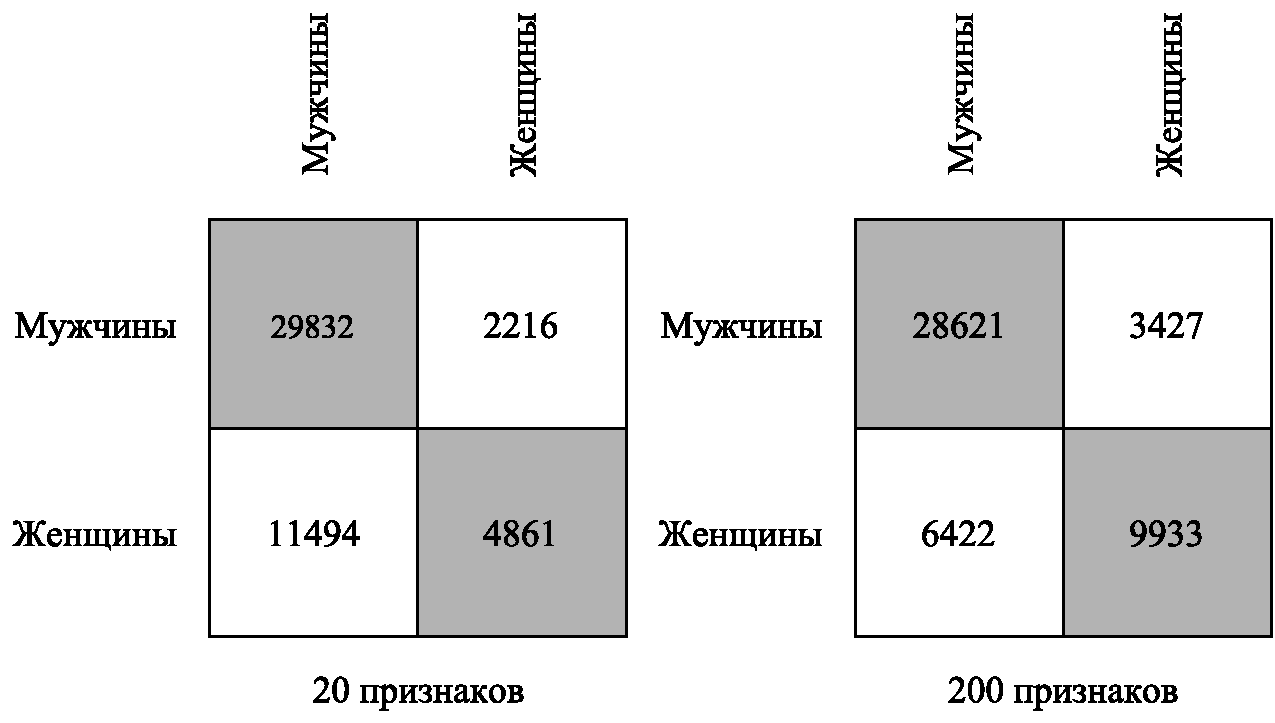
\includegraphics[scale=0.75]{figs/order-lsa-confusion.pdf}
\end{figure}

В таблице~\ref{tab:bow_we} приведены результаты эксперимента
с применением подхода <<bag of words>> и метода word embedding.
Для модели, позволяющей получить лучшие результаты в задаче
определения пола пользователей на рисунке~\ref{fig:bow_we_conf}
приведены матрицы ошибок.

\begin{table}[!h]
    \caption{Результаты эксперимента с применением подходов
            <<bag of words>> и word embedding}
    \label{tab:bow_we}
\centering
\begin{tabular}{|c|c|c|c|c|}\hline
    \textbf{Формула} & \boldmath$l(x)$ & \boldmath$g(x)$ & \textbf{Определение пола} & \textbf{Определение возраста} \\\hline
    \multicolumn{5}{|c|}{\textbf{20 признаков}} \\\hline
    TF-IDF & $1$ & $1$ & 79,59\% & 3,14 \\\hline
    TF-IDF & $\log{x}$ & $1$ & 79,32\% & 3,15 \\\hline
    TF-IDF & $\log{x}$ & $\log{x}$ & 78,06\% & 3,43 \\\hline
    TF-IDF & $\log{x}$ & $\sqrt{x}$ & 78,04\% & 3,43 \\\hline
    TF-IDF & $\sqrt{x}$ & $1$ & 78,33\% & 3,34 \\\hline
    TF-IDF & $\sqrt{x}$ & $\log{x}$ & 78,05\% & 3,43 \\\hline
    TF-IDF & $\sqrt{x}$ & $\sqrt{x}$ & 78,01\% & 3,43 \\\hline
    TF-IDF & $x$ & $1$ & 78,12\% & 3,40 \\\hline
    TF-IDF & $x$ & $\log{x}$ & 78,00\% & 3,43 \\\hline
    TF-IDF & $x$ & $\sqrt{x}$ & 78,00\% & 3,43 \\\hline
    log-entropy & --- & --- & \textbf{81,91\%} & \textbf{2,84} \\\hline
    \multicolumn{5}{|c|}{\textbf{200 признаков}} \\\hline
    TF-IDF & $1$ & $1$ & 78,98\% & 3,24 \\\hline
    TF-IDF & $\log{x}$ & $1$ & 78,26\% & 3,20 \\\hline
    TF-IDF & $\log{x}$ & $\log{x}$ & 78,05\% & 3,42 \\\hline
    TF-IDF & $\log{x}$ & $\sqrt{x}$ & 78,01\% & 3.43 \\\hline
    TF-IDF & $\sqrt{x}$ & $1$ & 78,21\% & 3,38 \\\hline
    TF-IDF & $\sqrt{x}$ & $\log{x}$ & 78,03\% & 3,43 \\\hline
    TF-IDF & $\sqrt{x}$ & $\sqrt{x}$ & 78,01\% & 3,43 \\\hline
    TF-IDF & $x$ & $1$ & 78,12\% & 3,41 \\\hline
    TF-IDF & $x$ & $\log{x}$ & 78,01\% & 3,43 \\\hline
    TF-IDF & $x$ & $\sqrt{x}$ & 78,00\% & 3,43 \\\hline
    log-entropy & --- & --- & \textbf{83,86\%} & \textbf{2,65} \\\hline
\end{tabular}
\end{table}

\begin{figure}[!h]
\caption{Матрицы ошибок для задачи определения пола с
         применением подходов <<bag of words>> и
         word embedding}
\label{fig:bow_we_conf}
\centering
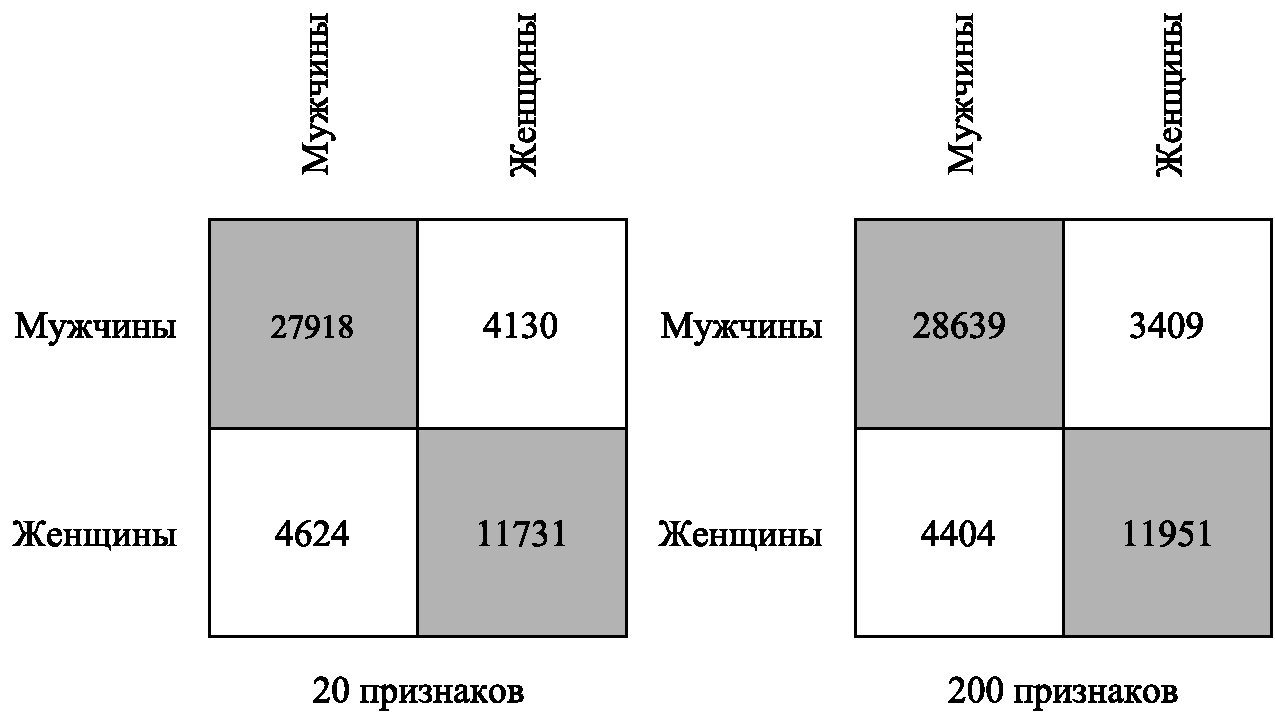
\includegraphics[scale=0.75]{figs/bow-we-confusion.pdf}
\end{figure}

В таблице~\ref{tab:order_we} приведены результаты
экспериментов с применением подходов вычисления матрицы
<<исполнитель-пользователь>> на основе порядка следования
исполнителей и word embedding. Для модели, позволяющей
достигнуть лучших результатов, на рисунке~\ref{fig:order_we_conf}
приведены матрицы ошибок.

\begin{table}[!h]
    \caption{Результаты эксперимента с применением подходов
             вычисления матрицы <<исполнитель-пользователь>>
             на основе порядка следования исполнителей 
             и word ebmedding}
    \label{tab:order_we}
\centering
\begin{tabular}{|c|c|c|}\hline
    \boldmath$f(a)$ & \textbf{Определение пола} & \textbf{Определение возраста} \\\hline
    \multicolumn{3}{|c|}{\textbf{20 признаков}} \\\hline
    $\frac{1}{\log(a + 1)}$ & 80,38\% & 2,98 \\\hline
    $\frac{1}{\sqrt{a}}$ & \textbf{81,55\%} & \textbf{2,90} \\\hline
    $\frac{1}{a^2}$ & 72,27\% & 4,64 \\\hline
    $\frac{1}{a}$ & 78,92\% & 3,75 \\\hline
    $51 - a$ & 77,90\% & 3,48 \\\hline
    $\log{51} - \log{a}$ & 78,11\% & 3,39 \\\hline
    $\sqrt{51} - \sqrt{a}$ & 78,15\% & 3,42 \\\hline
    \multicolumn{3}{|c|}{\textbf{200 признаков}} \\\hline
    $\frac{1}{\log(a + 1)}$ & 78,56\% & 3,15 \\\hline
    $\frac{1}{\sqrt{a}}$ & 80,32\% & \textbf{2,99} \\\hline
    $\frac{1}{a^2}$ & 74,77\% & 4,42 \\\hline
    $\frac{1}{a}$ & \textbf{80,89\%} & 3,35 \\\hline
    $51 - a$ & 77,82\% & 3,49 \\\hline
    $\log{51} - \log{a}$ & 78,18\% & 3,40 \\\hline
    $\sqrt{51} - \sqrt{a}$ & 78,11\% & 3,42 \\\hline
\end{tabular}
\end{table}

\begin{figure}[!h]
\caption{Матрицы ошибок для задачи определения пола с
         применением подходов вычисления матрицы 
         <<исполнитель-пользователь>> на основе порядка следования
         исполнителей и word embedding}
\label{fig:order_we_conf}
\centering
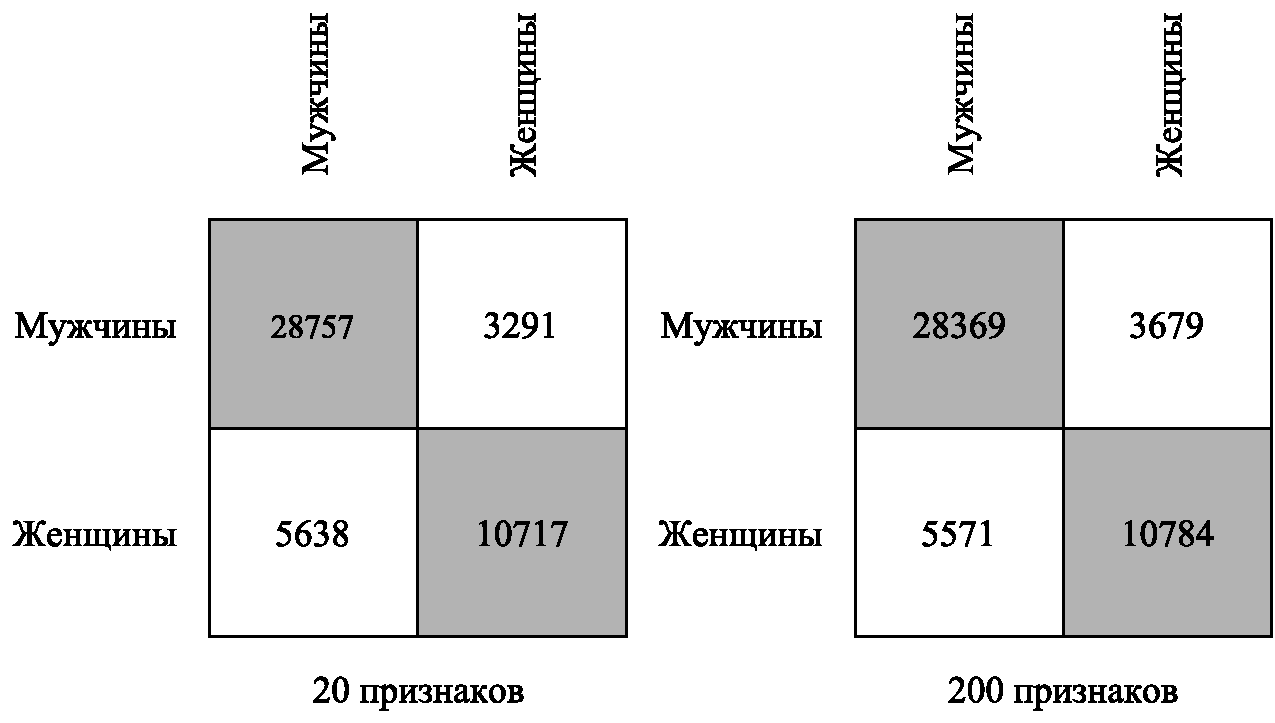
\includegraphics[scale=0.75]{figs/order-we-confusion.pdf}
\end{figure}

Как видно из результатов, подход к снижению размерности
матрицы <<исполнитель-пользователь>> на основе <<word embedding>>
позволяет достигать приемлемых результатов при малом числе признаков.
Напротив, подход, основанный на латентном семантическом анализе,
позволяет получить хорошие результаты только при использовании
достаточно большого числа признаков.

Также следует отметить, что подход на основе <<word embedding>>
позволяет решать задачу определения возраста пользователей сильно
лучше, чем подход на основе латентного семантического анализа.

Подход к вычислению матрицы <<исполнитель-пользователь>> на
основе порядка следования исполнителей в некоторых случаях
даёт улучшение результата, но наилучший результат получается
при применении формулы log-entropy в комбинации с word embedding.

Наконец, в таблице~\ref{tab:total_results} приведены итоговые
результаты эксперимента. Колонка таблицы \textit{BOW + word embedding}
показывает наилучшие результаты, достигнутые при использовании
подхода <<bag of words>> при вычислении матрицы <<исполнитель-пользователь>>
и подхода к снижению размерности матрицы на основе техники
word embedding, предложенного в рамках настоящей работы. В колонке
\textit{BOW + ЛСА} указаны лучшие результаты, достигнутые при
использовании стандартного подхода на основе <<bag of words>>
и латентного семантического анализа. В колонке \textit{baseline}
приведены результаты, достигнутые в исследовании~\cite{wu2014gender}.
Как видно, полученные результаты при использовании предложенного подхода
несколько превосходят результаты, полученные при использовании
стандартного подхода, и результаты, достигнутые ранее.

\begin{table}[!h]
    \caption{Итоговые рузультаты}
    \label{tab:total_results}
\centering
\begin{tabular}{|c|c|c|c|}\hline
    \textbf{Задача} & \textbf{BOW + word embedding} & \textbf{BOW + ЛСА} & \textbf{baseline} \\\hline
    Определение пола & \textbf{83,86\%} & 82,46\% & 78,87\% \\\hline
    Определение возраста & \textbf{2,65} & 3,54 & 3,69 \\\hline
\end{tabular}
\end{table}

Стоит отметить, что размерность пространства признакового описания
пользователей в эксперименте была выбрана произвольным образом. Выбор
других значений для размерности пространства признакового
описания может сильно влиять на результат.

Также следует отметить, что значения параметров алгоритмов классификации и
регрессии, выбор которых иногда сильно влияет на результат, настраивались
не самым оптимальным образом. Возможно, выбор <<сетки параметров>> в
алгоритме GridSearchCV с использованием рекомендации из
статьи~\cite{hsu2003practical} позволил бы достичь более хороших результатов.
Кроме того, для настройки параметров алгоритмов машинного обучения
могут быть использованы более мощные методы такие как 
\textit{gradient-based hyperparameter optimization}~\cite{maclaurin2015gradient}
и \textit{bayesian optimization}~\cite{hutter2011sequential}.

\section{Дополнительный эксперимент}

Описанный подход в разделе~\ref{ch:problem_solving} может быть также
применён и в других задачах, в которых присутствуют текстовые данные.
В данном разделе описан дополнительный эксперимент, проведённый
для апробирования предложенного подхода на задаче \textit{Bag of
Words Meets Bags of 
Popcorn}\footnote{https://www.kaggle.com/c/word2vec-nlp-tutorial} с
сайта \textit{Kaggle.com}\footnote{https://www.kaggle.com}.

Данная задача является задачей бинарной классификации текстовых документов.
Обучающая выборка включает в себя как документы, у которых
присутствуют метки классов, так и те, у которых они отсутствуют.
Для построения модели использовались только документы обучающей
выборки, у которых имеются метки классов. 

Матрица <<термин-документ>> вычислялась на основе формулы 
log-entropy. Алгоритм LSI использовался с параметром
\textit{num\_topics} равным 300. Алгоритм Word2Vec
использовался с параметрами \textit{size} = 300 и \textit{window} =
10. В качестве алгоритма классификации был использован алгоритм
\textit{LogisticRegressionClassifier} с 
параметром \textit{class\_weight} = \textit{auto} из
библиотеки \textit{gensim}. Термины из документов извлекались
с помощью программной библиотеки \textit{nltk}~\cite{nltk}.

Для модели на основе LSI достигнутый
результат равен 0{,}86660, для модели на основе Word2Vec~---
0{,}88048. Результат является площадью под
ROC-кривой. Как видно, предложенный подход показал
приемлемый результат и для данной задачи.


\chapterconclusion

В настоящей главе был описан эксперимент, который был проведён
в рамках исследования для апробирования предложенного подхода.

На примере задачи определения пола и
возраста пользователей сайта Last.fm на основе анализа их
музыкальных предпочтений была продемонстрирована
состоятельность предложенного подхода.

В данной конкретной задаче подход к вычислению матрицы
<<исполнитель-пользователь>> не дал улучшения результата по
сравнению со стандартным подходам на основе предположения
<<bag of words>>.

Напротив, предложенный подход векторного представления пользователей
с использованием линейной комбинации векторов, полученных
посредством техники word embedding позволяет достигнуть
значительного улучшения результата по сравнению со стандартным
походом на основе латентного семантического анализа. Кроме того,
предложенный подход позволяет получать приемлемые результаты
при малой размерности пространства признакового описания пользователей.

